%*******************************************************************************
%****************************** Second Chapter *********************************
%*******************************************************************************
% !TEX root = ../thesis.tex
\chapter{Literature Review}
\label{ch:litReview}
\ifpdf
    \graphicspath{{Chapter2/Figs/Raster/}{Chapter2/Figs/PDF/}{Chapter2/Figs/}}
\else
    \graphicspath{{Chapter2/Figs/Vector/}{Chapter2/Figs/}}
\fi

\section{Introduction}
Because of the complex and dynamic nature of mass gathering events, crowd monitoring is playing an increasing important role in emergency management for mass gathering. As the current practised crowd monitoring techniques are resource intensive and prone to error, much effort has been done to automate the crowd monitoring process. This chapter will review the state-of-art crowd monitoring techniques in the literature in order to identify the gaps as well as to assess the potential of using those techniques in crowd monitoring.

Although most of these novel approaches were capable to detect the critical condition in the crowd by applying quantitative reasoning, they lacked a model that can represent and distinguish between different crowds. In fact, making the distinction between different crowds is the key factor in emergency management to prevent losses of life, health, property and money \citep{Berlonghi1995}. The lack of model also made it difficult for existing approaches to incorporate the newly available information sources and sensing techniques in context aware computing. Therefore, this chapter will also discuss the investigate crowd models in the literature of a wide range of research areas.

This chapter is structured as follow. Firstly, the current approaches in crowd monitoring will be introduced, followed by our analysis and discussion. Secondly, another literature review on crowd modelling will be discussed. The chapter ends with a conclusion which summarises our findings.

\section{Current Approaches in Crowd Monitoring}
Most research regarding crowd monitoring have focused on the vision-based approach where computers were used to automatically analyse the recorded video to detect the abnormal and potentially dangerous crowd situations. More recent novel approaches leveraged the power of mobile devices and mobile crowdsensing to monitor the crowd, including sensory data analysis and real-time social media analysis. The following section will look further into each area of current methods in crowd monitoring. 

\subsection{Computer Vision}
The objective of this area of approach is to enable computers to acquire and analyse the recorded video to replace human operators in crowd monitoring. The first advantage is the reusability the existing CCTV systems to support both data collection and online monitoring. One of the pioneer vision-based approaches was from \citet{Davies1995}. They proposed a crowd monitoring system where the images captured from all cameras are processed by a centerised computer to identify crowd problems as soon as they arise and alert the operators. The algorithm involving the background removal and the edge detection was capable to estimate the density of the crowd while the motion can be detected by the optical flow computation.

\citet{Marana1997} argued against the accuracy of the edge detection method mentioned above to estimate the number of people in a high density crowd. They proposed different texture analysis techniques such as GDLM based on the grey level in the image, Fourier spectrum and Minkowski fractal dimension \citep{Marana1999} to classify the density of the crowd into five different levels: very low, low, moderate, high and very high density. Different classifiers were evaluated such as neural network, Bayesian network and fitting function and statistical Bayesian classifier appeared to produce highest accuracy \citep{Marana1998}.

In the context of public transport safety, \citet{Velastin1999} pointed out the dangerous situations in a crowd including the overcrowding and the abnormal movement. They also applied image processing techniques to analyse CCTV recordings in an acceptable rate for the real-time detection of crowded situation.

Video analysis was also employed to maintain the safety of massive event in \citet{Johansson2008}’s work based on the theory of crowd turbulence. Image processing was also utilised in abnormality detection in crowded scene \citep{Mahadevan2010, Mehran2009}. \citet{Mehran2009} further improved the optical flow method by incorporating the Social Force Model, which used the force flow between each individual to illustrate the crowd behaviour in order to identify the abnormal behaviour. Other vision-based approaches that can be mentioned are crowd segmentation and counting by \citet{Chan2008} and density estimation by \citet{Li2010}.

\citet{Andersson2009} pointed out the common problems in analysis of CCTV are their incompetent performance with low light conditions and shadow effects. Therefore, thermal infrared imaging was introduced as a robust solution to enhance the visibility. Since infrared cameras operate in long wave infrared band, they can capture heat emitted from an object which temperature lies within -30 to 100 degrees Celsius. Although, thermal image processing requires special equipment to be installed, the new generation of the low cost un-cooled infrared cameras have enabled the application of this method in crowd monitoring. ICAPS project \citep{Pham2007} utilizes thermal imaging to detect potential threats on subway platforms by watching for people lying on the ground.

A combination of both visual image and thermal image as the context sources was proposed by \citet{Andersson2009}. Based on the amount of motion activity, the movement and the size of the crowd, abnormal behaviour of the crowd can be identified. In addition to visual cameras and infrared cameras, \citet{Yaseen2013} introduced the use of light intensity and temperature sensors in a sensory fusion approach. These additional sensors were used to measure the ambient light condition and the temperature to remove noise during the image processing.

\subsection{Sensory Data Analysis}
As mentioned before, in the sensory fusion model proposed by \citet{Yaseen2013}, the light intensity and temperature sensors can be used to give the knowledge about the surrounding environment. Although they only played insignificant role in this research, the idea of gathering and analysing context data collected from sensors has been well adopted in a number of researches thanks to the development of mobile technology.

One of the most notable works to be mentioned is \citet{Wirz2012}’s CoenoSense framework. By highlighting several limitations of vision-based approach such as the limited field of view or the impact of obstacles and lighting condition, they presented a real-time crowd monitoring method using GPS information collected from the mobile phones of participants. The CoenoSense data collection framework relied on a mobile application served as a probe to regularly sampling the current GPS location of the mobile phone \citep{Wirz2013}. With the assumption that the distribution of application's users corresponds to the actual distribution of the participants, their location traces can be used to measure the approximate density and movement of the crowd, enabling the crowd turbulence and crowd pressure to be calculated accordingly. The visualisation of the crowd distribution, movement, turbulence and pressure as a heat-map received positive feedbacks from the police and emergency team as this method had certain advantages over the traditional CCTV monitoring. For example, it provided an overview and intuitive look of the crowd condition.

CoenoSense has proven the feasibility of using the sensor-enhanced mobile phones in participatory sensing. Another type of built-in sensor that can be employed in participatory sensing is Bluetooth \citep{Stopczynski2013,Weppner2011,Weppner2013}. \citet{Weppner2011} proposed a collaborative crowd density estimation method using Bluetooth enabled phones. Instead of relying on fixed scanners, a software module installed on the participants’ phones scanned for the presence of other devices within its vicinity. Apart from the number of discovered devices, the signal strength was also taken into account as the density level of crowd would affect the pattern of signal. \citet{Weppner2013} incorporated GPS information to track the movement of a dynamic crowd. The result of analysis was seven levels of crowd density from nearly empty to extremely high.

\citet{Roggen2011} investigated the possibility of employing the accelerometers to recognise the crowd behaviours. The pattern of sensory data collected by on-body sensors were analysed and clustered to identify individual behaviour and the basic group behaviour. Because the on-body sensors in their experiment worked similarly to the accelerometer integrated in common mobile phones, this approach can be practised with mobile phone sensors.

Interestingly, sensory data analysis can also include sound as an information source. Although these approaches were not explicitly defined for any specific domain, there is a potential use for crowd monitoring. As speech can be considered as a fingerprint of a person, Crowd++ proposed by \citet{Xu2013} was a platform which leveraged the microphone in mobile phones to detect the speech and count the number of different speakers in a place. \citet{Kannan2012} designed a peer-to-peer (P2P) multi-hop network of microphone where each node transmitted and received inaudible sound to a surrounding node via microphone and speaker respectively to automatically update the number of devices in the network. This method had the advantage of easy deployment, scalability and energy efficiency while keeping the minimal interference and achieving a high accuracy in counting the number of people in the crowd.

According to \citet{Ramesh2014}, smart context sources can be collected from two categories of sensors. These included the hard sensors and the soft sensors. Hard sensors might include accelerometers, digital compasses, gyroscopes and location sensors while soft sensors referred to the user generated content from SNS sites. They proposed a multi context based approach for the mitigation of crowd disaster. The system consisted of two sensing modules: a wireless multimedia sensing module and a smart-phone sensing module. The former included temperature sensors, visual cameras and acoustic sensors while the latter consisted of mobile phone sensors such as accelerometers, gyroscopes and location sensors. The module was installed in the form of a mobile application. The system was able to recognise several activities of the individual in the crowd and predict the possibility of human stampede.

\subsection{Social Media Analysis}
As mentioned above, the social media such as SNS can be categorised as a soft sensor in mobile sensing. However, the technique and the process of social media analysis is very different from other sensory data analysis. The underlying technique of social media analysis is the sentiment analysis which purpose is to identify the polarity of opinion in a text. Twitter is frequently used as the information source in research on social media analysis because the data can be easily accessed by an Application Programming Interface (API). Many studies have been conducted on the behaviour of Twitter users during emergency events \citep{Hughes2009,Sakaki2010,Vieweg2010,Yin2012}.

In the context of crowd monitoring, \citet{DelirHaghighi2013} proposed a real-time crowd monitoring system based on the sentiment analysis of Twitter streams. The system was able to identify negative moods in the crowd by analysing tweets about a specific event and visualise the mood of the crowd.

\subsection{Analysis and Discussion}
The state-of-art crowd monitoring techniques mentioned above have showed the potential of capturing and analysing contextual data to detect potentially emergency situation in the crowd. In order to fully understand the strength and limitation of these techniques, they will be analysed under following criteria.

\begin{itemize}
	\item \textbf{Domain/Application} - the domain or the application where the monitoring technique is used is important because each domain emphasises on certain characteristics. 
	\item \textbf{Underlying technique} - image processing, sensory data analysis or social data analysis.
	\item \textbf{Context data/ Information source} - the source where contextual data is collected, such as CCTV records, GPS, mobile phone built-in sensors or social networks. Information source is important because it affects the feasibility to collect data in different environments.
	\item \textbf{Processing} - whether this analysis can be processed in real-time or in batch. Real-time is essential for emergency management during the event while batch analysis is more suitable in post-event stage.
	\item \textbf{Venue type} - whether the monitored crowd is outdoor or indoor. This is because an indoor monitoring can make use of the existing equipment such as installed CCTV system while an outdoor monitoring cannot.
\end{itemize}

Table \ref{table:crowdMonitoringTechAnalysis} analyses existing crowd monitoring approaches according to above criteria.

\begin{center}
	\begin{longtable}{|p{2cm}|p{2.5cm}|p{2.5cm}|p{2cm}|p{1.5cm}|p{2cm}|}
		\caption{Comparative analysis of crowd monitoring techniques}
		\label{table:crowdMonitoringTechAnalysis} \\
		\hline
		\textbf{Work} & \textbf{Domain / application} & \textbf{Analysis technique} & \textbf{Context data} & \textbf{Process} & \textbf{Venue} \\
		\hline \hline
		\citet{Davies1995} & Pedestrian engineering & Image processing & CCTV & Realtime & Outdoor and Indoor \\
		\hline
		\citet{Marana1997} & Crowd monitoring (Density estimation) & Image processing (Texture analysis and classifier from texture to density) & CCTV & Realtime & Outdoor and Indoor \\
		\hline
		\citet{Velastin1999} & Public transport safety & Image processing & CCTV & Realtime & Outdoor and Indoor \\
		\hline
		\citet{Johansson2008} & Mass event safety (Post event analysis) & Image processing & Video & Batch (Post event) & Outdoor and Indoor \\
		\hline
		\citet{Mehran2009} & Transportation and public safety & Image processing (Social Force Model and Bag of Words) & Video & Realtime & Outdoor and Indoor \\
		\hline
		\citet{Mahadevan2010} & Temporal and spatial anomaly detection & Image processing (Mixture of dynamic texture analysis) & Video & Realtime & Outdoor and Indoor \\
		\hline
		\citet{Chan2008} & Crowd counting & Image processing (Mixture of dynamic texture to crowd segmentation, Gaussian process regression to estimate number) & Video & Realtime & Outdoor and Indoor \\
		\hline
		\citet{Li2010} & Density estimation & Image processing (Background removing, neural network classifier from texture to density) & Video & Realtime & Outdoor and Indoor \\
		\hline
		ICAPS \citep{Pham2007} & Public safety & Image processing & Thermal image & Realtime & Indoor \\
		\hline
		\citet{Andersson2009} & Public safety & Image processing & Sensor fusion of CCTV and thermal image & Realtime & Outdoor and Indoor \\
		\hline
		\citet{Yaseen2013} & Large event safety (Density estimation) & Image processing & Sensor fusion of CCTV and thermal image, light and temperature sensor& Realtime & Outdoor and Indoor \\
		\hline
		CoenoSense \citep{Wirz2012} & Mass gathering security & Sensory data analysis & GPS (mobile phone) & Realtime & Outdoor and Indoor \\
		\hline
		Crowd++ \citep{Xu2013} & Event planning (Crowd size estimation and social hotspot discovery) & Audio processing (Speech recognition) & Microphone (mobile phone) & Realtime & Indoor\\
		\hline
		\citet{Kannan2012} & Public transport planning and  event planning (Crowd size estimation) & Audio processing (Inaudible, P2P communication in multi-hop network) & Microphone (mobile phone) & Realtime & Outdoor and Indoor \\
		\hline
		\citet{Weppner2011} & Participatory sensing in massive event (Density estimation) & Sensory data analysis (Discovery of device and signal strength analysis) & Bluetooth enabled sensor (mobile phone) & Batch & Outdoor and Indoor \\
		\hline
		\citet{Weppner2013} & Participatory sensing in massive event (Density estimation) & Sensory data analysis (Discovery of device and signal strength analysis) & Bluetooth enabled sensor and GPS (mobile phone) & Batch & Outdoor and Indoor \\
		\hline
		\citet{Stopczynski2013} & Participatory sensing in massive event & Sensory data analysis (Discovery of Bluetooth unique identifier) & Bluetooth enabled sensor and GPS (mobile phone) & Batch & Outdoor and Indoor \\
		\hline
		\citet{Roggen2011} & Crowd behaviour recognition & Sensory data analysis (Sensory pattern analysis and graph clustering) & On body accelerometer & Realtime & Outdoor and Indoor \\
		\hline
		\citet{Ramesh2014} & Disaster mitigation & Sensory data analysis & Wireless sensors and mobile sensors & Realtime & Outdoor and Indoor \\
		\hline
		\citet{DelirHaghighi2013} & Emergency management & Social media analysis (Sentiment analysis) & Social media (Twitter) & Realtime & Outdoor and Indoor \\
		\hline
	\end{longtable}
\end{center}

The advantage of the vision-based approaches is the reusability of existing CCTV system which is deployed in most buildings and metropolitan areas. However, as mentioned by \citet{Davies1995}, because most cameras are installed for security reasons, they are often not located in the best position to collect data for crowd monitoring. Moreover, CCTV monitoring might be affected by obstacles, and most importantly, it heavily relies on a good lighting condition \citep{Wirz2012}. Although thermal infrared camera could overcome those issues, special hardware need to be installed. Another limitation is the capability of vision-based approach to monitor large scale mass gathering. Firstly, installing camera in most open areas is not practical. Secondly, as pointed out by \citet{Wirz2012}, it is difficult to fuse information from many cameras to obtain global situational awareness.

Sensory data analysis leverages the power of mobile crowdsensing which is being made feasible by the high distribution of sensor enhanced smart phones in the society. Related works mentioned above have demonstrated that a variety of mobile sensors such as GPS, Bluetooth enabled sensors and microphones can be used as the source of contextual data for crowd monitoring. Each sensor has its own pros and cons in different operating environment, for example, a GPS sensor works well outdoors, yet is limited in indoor or underground use due to satellite signal obstruction of ceilings and walls. On the other hand, the audio-based approach seems feasible for indoor environment but might be subject to noise.

The idea of a framework integrating multiple sensors was discussed by \citet{Ramesh2014}, whose work suggested the possibility of integrating SNS as a soft sensor. Although social media was not implemented into their proposed system, the advantage of using social media analysis to get the global situation of a crowd in crowd monitoring has been proven by another work by \citet{DelirHaghighi2013}.

Finally, most of the above mentioned crowd monitoring systems relied solely on an analysis method over collected data to identify a particular problem in the crowd. However, they lacked a model that can distinguish different moods, behaviours and types of the crowd which is crucial in the context of emergency management. Therefore, in the next section, existing works on crowd modelling in the literature will be investigated.

\section{Crowd Model}
\citet{Berlonghi1995} emphasized on the importance of making the distinctions of diffrent crowd types in crowd control and crowd management because operations relying on random judgments might lead to serious losses of life, money or property. In spite of its significance, very little research has been done on crowd typologies. An intensive literature review carried out by \citet{Challenger2009} showed only two related publications from \citet{Momboisse1967} and \citet{Berlonghi1995}.

This section will cover those two works and also consider the relevant studies in a broader area of research such as crowd psychology, sociology and crowd dynamics as well as incorporate views from the military and police literature regarding classification of crowd. These classifications are grouped into two groups based on their approaches. The first subsection focuses on the models that utilise internal factors of the crowd, such as the behaviour or mood to make the distinction. The second subsection will discuss other classifications based on external characteristics, for example, the movement and the density of the crowd.

\subsection{Internal Characteristics Modeling}

From the sociology perspective, Herbert Blumer was among the first sociologists who put forward the term ``collective behaviour'' which referred to human behaviour in a group \citep{Blumer1951}. He defined four forms of collective behaviour (Table \ref{table:blumerCrowdType}) based on their emotional intensity \citep{Imhonopi2013}. Blumer’s theories has become the baseline in police training material and literature \citep{Schweingruber2000}. Another type of the crowd, a protest crowd, was later added to the above categories by later sociologists, which referred to a crowd that has a political goal \citep{Imhonopi2013}.

\begin{table}[!htbp]
	\caption{Blumer's four crowd types (Adopted from \citet{Imhonopi2013})}
	\label{table:blumerCrowdType}
	\centering
	\begin{tabular}{|l|p{10cm}|}
		\hline
		\textbf{Crowd type} & \textbf{Definition} \\ \hline \hline
		Casual & Loose collection of people who have litte interation \\ \hline
		Conventional & Result from delibrate planning of an event and conforming to norms appropriate to the situation \\ \hline
		Expressive & Form around an event that has emotional appeal \\ \hline
		Acting & Energetically doing something \\ \hline
	\end{tabular}
\end{table}

From the law enforcement point of view, \citet{Momboisse1967} also identified relatively similar four crowd types. He concentrated on the mob theory which suggested that any crowd can transform into a law breaking mob. His definitions of four crowd types are presented in Table \ref{table:momboisseCrowdType}. A hostile or aggressive crowd is considered to be most likely to turn into a mob.

\begin{table}[!htbp]
	\caption{Momboisse's four crowd types (Adopted from \citet{Schweingruber2000})}
	\label{table:momboisseCrowdType}
	\centering
	\begin{tabular}{|l|p{10cm}|}
		\hline
		\textbf{Crowd type} & \textbf{Definition} \\ \hline \hline
		Casual & Happen to be present at a given place but are not unified or organized \\ \hline
		Conventional & Assembled for a specific purpose, such as witnessing a ball game, parade, play or fire 
		and have similar common interest \\ \hline
		Expressive & Involve in expressive behaviour, such as dancing or singing, but not directed in a destructive way \\ \hline
		Acting & Unorganized throng willing to be led into lawlessness, but hesitant because lacking organization, courage and unity of purpose \\ \hline
	\end{tabular}
\end{table}


According to \citet{Momboisse1967}, the key difference between a mob and a crowd is the awareness and willingness to follow the law and order since a mob is not law-abiding. In his theory, mob is then further considered and categorized into four types (Table \ref{table:momboisseMobType}). As can be seen from the terminology and definition, there is little distinction between an expressive crowd which is neutral and an expressive mob which might pose potential danger.

\begin{table}
	\caption{Momboisse's four mob types (Adopted from \citet{Schweingruber2000})}
	\label{table:momboisseMobType}
	\centering
	\begin{tabular}{|l|p{10cm}|}
		\hline
		\textbf{Mob type} & \textbf{Definition} \\ \hline \hline
		Escapist & Motivated to flee from a real or imagined threat \\ \hline
		Acquisitive &  Motivated by the desire to acquire something \\ \hline
		Expressive & Engage in expressive bahaviour \\ \hline
		Aggressive & Include race riots, lynching and prison riots. It aims to destroy persons or property \\ \hline
	\end{tabular}
\end{table}


Momboisse’s work was broadly adopted in police literature because it classified a crowd by its behaviour and motivation which are the factors of greatest interest from the perspective of law enforcement \citep{FBI1967}. Based on the mob theory, the Federal Bureau of Investigation (FBI) looked further into the mob and was able to distinguish seven types of people involving in a mob by their attitude toward violence. Table \ref{table:fbiMobBehavior} presents those seven observable behaviours in a mob scene, six of which are involved in violent activities while resisters are against violence.

\begin{table}
	\caption{FBI's seven behaviour in a mob (Adopted from \citet{FBI1967})}
	\label{table:fbiMobBehavior}
	\centering
	\begin{tabular}{|l|p{10cm}|}
		\hline
		\textbf{Mob member} & \textbf{Definition} \\ \hline \hline
		Impulsive and lawless & Start the riot the incite others to violence \\ \hline
		Suggestive &  Easily influenced to follow the lead of more violent \\ \hline
		Cautious & Would like to get into the fracas but wait for the cloak of anomity \\ \hline
		Yielders & Do not join the action until the larger number of persons participating gives the impression of universality \\ \hline
		Supportive & Enjoy the show and even shout encouragement \\ \hline
		Psychopathic & Angry at the world \\ \hline
		Resisters & Oppose to violence \\ \hline
	\end{tabular}
\end{table}

Similarly, crowd behavioural modelling is considered to play an increasingly significant role by the military. The cognitive crowd model consisting of aggressive, escapist, acquisitive and expressive types was also applied in military researches to simulate crowd behaviour in combat situation \citep{Petty2004}. In this application, \citet{Nguyen2005} simplified the cognitive representation to a single state called the aggression level which consisted of personal aggression level, group aggression level and crowd aggression level. These aggression levels can range from neutral, avoidance, curious non-aggressive, aggressive, aggressive non-lethal to violent lethal. However, to be applied in emergency management, more mental states must be considered \citep{Zhou2010}.

In social psychology, there have been several works on the classification of the crowd. In the book ``Mass phenomena'', \citet{Brown1954} divided a crowd into two main categories that were the audience and the mob. An audience was defined as a passive crowd while a mob was described as an active crowd. These categories were then further broken down based on their purpose and feeling \citep{Pelechano2008}, which formed a hierarchical taxonomy as illustrated in Figure \ref{fig:brownCrowdType}.

\begin{figure}[!htbp] 
	\centering    
	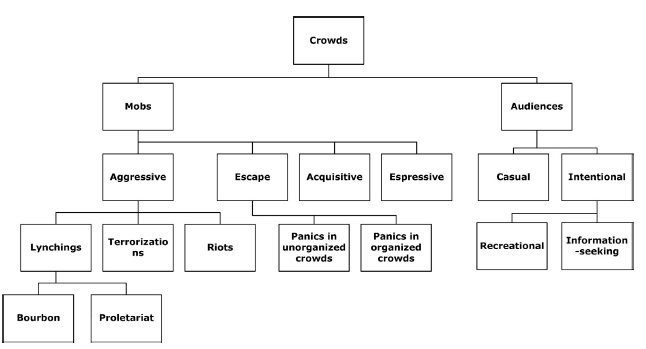
\includegraphics[width=1.0\textwidth]{BrownCrowdType}
	\caption{Brown's taxonomy of crowd (Adopted from \citet{Pelechano2008})}
	\label{fig:brownCrowdType}
\end{figure}


According to Brown’s definition, aggressive crowds are determined by anger while escapist crowds are by fear. Acquisitive and expressive types are classified by the motivation which are acquiring objects or expressing a purpose respectively \citep{Durupinar2010}.

\citet{Forsyth2009} has defined a relatively similar classification of the crowd, which also distinguished a crowd into a gathering and a mob. Figure \ref{fig:forsythCrowdType} illustrates the branching of crowd classification. The difference between this Forsyth’s hierarchy and Brown’s hierarchy mentioned above is that escapist and acquisitive crowds are classified under panics in Forsyth's classification. 

\begin{figure}[!htbp]
	\centering    
	\includegraphics[width=1.0\textwidth]{ForsythCrowdType}
	\caption{Forsyth's classification of crowd (Adopted from \citet{klupfel2005models})}
	\label{fig:forsythCrowdType}
\end{figure}

The idea of using emotion, such as \textit{fear} and \textit{anger}, in order to distinguish different crowds was also adopted by other sociologists \citep{Lofland1985,Smelser1998}. Three basic fundamental emotions of humans that are \textit{fear}, \textit{joy} and \textit{anger} can express three corresponding forms of a crowd \citep{Imhonopi2013}. Because collective behaviour is not limited by time and space, they also considered two types of crowds that are the compact crowd and the diffuse crowd, thus forming six different types of crowd (Table \ref{table:loflandCollectiveBehaviourType}). A compact crowd gathers at one particular place for the duration of a specific event whereas a diffuse crowd can be dispersed at different places and across time. An example of diffuse crowd is the collective behaviour on social media. Collective behaviour on social media might be interesting study, however, in our context of mass gathering, only compact crowds are considered to be relevant.

\begin{table}[!htbp]
	\caption{Lofland's six types of collective behaviour (Adopted from \citet{FBI1967})}
	\label{table:loflandCollectiveBehaviourType}
	\centering
	\begin{tabular}{|l|l|l|}
		\hline
		\textbf{Emotion} & \textbf{Crowd forms} & \textbf{Collective behaviour types} \\ \hline \hline
		\multirow{2}{*}{Expression of fear} & \multirow{2}{*}{Panic} & Compact \\
		& & Diffuse \\ \hline
		\multirow{2}{*}{Expression of joy} & \multirow{2}{*}{Craze} & Compact \\
		& & Diffuse \\ \hline
		\multirow{2}{*}{Expression of anger} & \multirow{2}{*}{Hostile outburst} & Compact \\
		& & Diffuse \\ \hline
	\end{tabular}
\end{table}

Elias Canetti was another author who has contributed a significant work on crowd behaviour. In Crowds and Power \citep{Canetti1962}, he defined four physical attributes of a crowd: growth, equality, density and direction. These external characteristics of the crowd will be discussed in detail in the next section. Looking at internal aspects of the crowd, Canetti identified five prevailing emotions in the crowd which produced five different crowd types: baiting, prohibition, reversal, feast and double \citep{McClelland2010}.

As mentioned earlier, another notable publication was the ``Understanding and planning for spectator crowds'' by \citet{Berlonghi1995} published in public safety science. It has been brought into practice by the emergency management planners in Australia \citep{EMA1999} and United States \citep{FEMA2005}. Table \ref{table:berlonghiCrowdType} illustrates eleven different crowd types identified by Berlonghi. This model was also adopted in \citet{DelirHaghighi2013a} and \citet{Arbon2007}’s ontology for case-based reasoning to predict the patient rate in a mass gathering.

\begin{table}
	\caption{Berlonghi's eleven crowd types (Adopted from \citet{Zeitz2009})}
	\label{table:berlonghiCrowdType}
	\centering
	\begin{tabular}{|l|p{8cm}|}
		\hline
		\textbf{Crowd type} & \textbf{Definition} \\ \hline \hline
		Ambulatory & Walking, usually calm  \\ \hline
		Disability / limited movement & Crowd has limited or restricted movement requires additional planning \\ \hline
		Cohesive / spectator & Watching a specific activity \\ \hline
		Expressive / revellous & Emotional release, for example, a cheering movement in unison \\ \hline
		Participatory & Involve in an actual event, for example, community fun runs \\ \hline
		Aggressive / hostile & Initially verbal, open to lawlessness \\ \hline
		Demonstrator & Organized to some degree, for example, pickets or marches \\ \hline
		Escaping / trampling & Danger may be real or imaginary \\ \hline
		Dense / suffocating & Reduction of individual physical movement \\ \hline
		Rushing / looting & Attempt to acquire, obtain, steal something, for example, tickets \\ \hline
		Violent & Attacking, terrorizing \\ \hline
	\end{tabular}
\end{table}

In reality, one crowd is expected to have multiple personalities \citep{Berlonghi1995}, therefore all of the above eleven types can exist as a group in a bigger crowd. This idea was also agreed by computer scientist in their recent researches in crowd simulation. Their works focused on simulating the heterogeneous crowd which consists of different, independent behaviour and characteristics. Based on Convergence Theory, the behaviour of the crowd is formed by the individuals; hence it is important to model the behaviour and interaction of the individuals in order to simulate a realistic, heterogeneous crowd behaviour \citep{Guy2011}.

Several approaches have been proposed which were derived from the personality trait theory. This theory implied that a personality trait can influence the behaviour, emotion and mental pattern of a person \citep{Durupinar2008}. The main objective of these researches was to map those traits with the low level parameters in simulation model to determine the behaviour of an individual agent, then observe the emerged global crowd behaviours. Two personality trait theories that were utilised are the PEN model \citep{Guy2011} and OCEAN model \citep{Durupinar2008,Durupinar2011}. The PEN model was constructed over three factors: Psychoticism, Extraversion, and Neuroticism while the OCEAN model consisted of Openness, Conscientiousness, Extroversion, Agreeableness and Neuroticism. The common adjectives to describe human personality were called the trait-descriptive adjectives, such as curious, alert, calm, rude were composed by different values of each of the above factors. Finally, they were mapped into corresponding parameters in the model as shown in Table \ref{table:oceanPersonality}.

\begin{table}[!htbp]
	\caption{Personality - trait - crowd model mapping (Adopted from \citet{Durupinar2008})}
	\label{table:oceanPersonality}
	\centering
	\begin{tabular}{|l|l|p{6.5cm}|}
		\hline
		\textbf{Model Parameter} & \textbf{OCEAN factor} & \textbf{Personality} \\ \hline \hline
		Leadership & E, A-, C+, N & Dominant, assertive, bossy, dependable, confident, unconfident, submissive, dependent, social, unsocial \\ \hline
		Trained / not trained & O & Informed, ignorant \\ \hline
		Communication & E & Social, unsocial \\ \hline
		Panic & N, C+ & Oversensitive, fearful, calm, orderly, predictable \\ \hline
		Impatience & E+, C, A & Rude, assertive, patient, stubborn, tolerant, orderly \\ \hline
		Pushing & A, E & Rude, kind, harsh, assertive, shy \\ \hline
		Right preference & A, C & Cooperative, predictable, negative, contrary, changeable \\ \hline
		Avoidance / personal space & E & Social, distant \\ \hline
		Waiting radius & A & Tolerant, patient, negative \\ \hline
		Waiting timer & A & Kind, patient, negative \\ \hline
		Exploring environment & O & Curious, narrow \\ \hline
		Walking speed & E & Energetic, lethargic, vigorless \\ \hline
	\end{tabular}
\end{table}

The simulation suggested that a low conscientiousness and agreeableness can lead to congestion during emergency evacuation and the non-conscientiousness and neuroticism was the root of panic in the crowd \citep{Durupinar2008}.

\subsection{External Characteristics Modeling}

Apart from the cognitive patterns, different crowds can also be distinguished by their external or physical characteristics which can be quantitatively measured. Several features of the crowd, such as the density, movement and flow rate can be utilised to identify different crowds in the context of crowd monitoring for emergency management.

As mentioned above, \citet{Canetti1962}’s theory also classified the crowd accordingly to their physical characteristics: growth, equality, density and direction. Each of these attributes identified a pair of crowd types. Derived from this theory, \citet{Bandini2011} formulated six types of crowds. Open and closed crowd were defined by their growth feature. Equality and density determined the stagnating or rhythmic types and movement classified a crowd into a slow or a quick crowd. \citet{Bandini2011} constructed an ontology approach to classify the crowd and defined a set of fuzzy rules mapping the features of the crowd with the six crowd types, as illustrated in Table \ref{table:bandiniCrowdType}.

\begin{table}[!htbp]
	\caption{Bandini's crowd type - feature mapping (Adopted from \citet{Bandini2011})}
	\label{table:bandiniCrowdType}
	\centering
	\begin{tabular}{|p{2.5cm}|p{1.5cm}|p{1.5cm}|p{2cm}|p{2cm}|p{1.5cm}|p{1.5cm}|}
		\hline
		\textbf{Crowd features} & \textbf{Open crowd} & \textbf{Closed crowd} & \textbf{Stagnating crowd} & \textbf{Rhythmic crowd} & \textbf{Slow crowd} & \textbf{Quick crowd} \\ \hline \hline
		Physical boundary & absent & present & & & & \\ \hline
		Psychological boundary & absent & present & & present & & \\ \hline
		Movement & & & absent & present & & \\ \hline
		Density & & & high/med & low & high/med & low \\ \hline
		Growth & high & med/low & & low & high & med/low \\ \hline
		Lifespan & & & & med/short & long & short \\ \hline
		Destination & & & & near & far & near \\ \hline
	\end{tabular}
\end{table}

From transportation engineering, \citet{Fruin1970} introduced the concept ``level of service'' to distinguish different crowds using the following features: the walking speed, the flow rate and the restriction \citep{Challenger2009}. This model has been adopted into the design and planning of pedestrian facilities \citep{Shiwakoti2008,Ye2008}. Six levels of service were defined, where a higher density increased the risk of pushing, falling, crushing and trampling.

Analysing the video footages of a crowd disaster during the Hajj in 2006, \citet{Helbing2007} claimed that density, the speed and flow of the crowd can be used as warning signs of potential accident. They coined the term ``crowd turbulence'' referring to the instabilities in the flow pattern of the pedestrians, which might trigger the trampling of people. According to their calculation, turbulence occurred when crowd pressure, which was the variance of speed multiplied by density, exceeded a certain threshold while the density of the crowd was high and the flow rate dropped below the critical threshold.

\citet{Lee2005} also studied the causes of past crowd accidents in different countries and discovered the relationship between density and crushing and trampling. Table \ref{table:densityCrushingTrampling} explained those two types of accidents and the critical density in the crowd which could lead to each situation. This research proved that a mathematical modelling of crowd motion can identify the dangerous locations for a crowd accident, hence a careful attention to those points can minimize the risk of trampling.

\begin{table}
	\caption{Crowd density leading to crushing and trampling}
	\label{table:densityCrushingTrampling}
	\centering
	\begin{tabular}{|l|p{9.5cm}|l|}
		\hline
		\textbf{Accident type} & \textbf{Definition} & \textbf{Density} \\ \hline \hline
		Trampling & High density with possible movement. Fatalities are caused by falling and being trampled & 5 ped/m2 \\ \hline
		Crushing & Extremely high density with almost impossible movement. Fatalities are caused by being compressed by pressure & 10 ped/m2 \\ \hline
	\end{tabular}
\end{table}

As mentioned in the previous section, crowd density was often used as a measure to monitor the safety of the crowd. Different crowds were classified by the level of density in the works by \citet{Marana1997} and \citet{Weppner2013} starting from very low density to very high density.

\subsection{Analysis and Discussion}

Psychological models \citep{Blumer1951,Lofland1985,Momboisse1967} were able to describe different crowd type based on the psychosocial domain of the crowd. Because reasoning was not clearly defined in those models, it would depend on the interpretation of the observer to determine whether a particular crowd type would pose a potential danger. This requires previous domain knowledge and experience that limit its use to the domain experts.

Simulation models using PEN \citep{Guy2011} and OCEAN \citep{Durupinar2008} personality trait theory were able to identify which personality of an individual can cause problems in evacuation. However, measuring individual’s personality is a difficult task.

Case-based reasoning in DO4MG \citep{DelirHaghighi2013a} considered both the psychological features and physical features of a crowd to predict the emergency situation. Case-based reasoning in general relied on historical data for prediction, therefore applying this method in crowd monitoring would be challenging when there is no access to similar data and some information required in the ontology cannot be captured in real-time.

The classification of crowd proposed by \citet{Lofland1985} and \citet{Smelser1998} suggested the importance of emotion as the motivation of the behaviour of a crowd. This idea was also agreed by \citet{Brown1954} whose taxonomy also used \textit{anger} and \textit{fear} to categorise the crowd.

Most of models which were capable of predicting the critical situations were based on the external characteristics of the crowd such as the density, size or movement \citep{Helbing2007,Lee2005}. This information can be obtained by sensors and the prediction can be made by quantitative reasoning. However, these models did not emphasise on the psychosocial factors which are important in emergency management.

\citet{Berlonghi1995}’s model has been broadly adopted as the guideline in emergency management. Comparing this model with other works from such authors as \citet{Blumer1951} or \citet{Momboisse1967}, it can be noticed that Berlonghi's model is also capable of representing the crowd types defined in other models. 

\begin{center}
	\begin{longtable}{|p{2.2cm}|p{2cm}|p{2cm}|p{4.2cm}|p{2.8cm}|}
	\caption{Comparison of different Crowd Models}
	\label{table:crowdModelComparison} \\
	\hline
	\multirow{2}{\linewidth}{\textbf{Crowd type}} & \multicolumn{3}{c|}{\textbf{Origin}} & \multirow{2}{\linewidth}{\textbf{Example}} \\
	\cline{2-4}
	& Crowd type & Source & Definition & \\
	
	\hline \hline
	\multirow{2}{\linewidth}{Ambulatory crowd} & Ambulatory \newline \newline & \citet{Berlonghi1995} & \multirow{2}{\linewidth}{People are walking in and out or to and from a venue \citep{Berlonghi1995}. Usually calm movement \citep{Zeitz2009}} & \multirow{2}{\linewidth}{People entering a stadium or a concert} \\
	\cline{2-3}
	& Casual crowd & \citet{Blumer1951} & & \\

	\hline
	\multirow{2}{\linewidth}{Limited movement crowd} & Disability / Limited movement \newline \newline & \citet{Berlonghi1995} & \multirow{2}{\linewidth}{People are limited or restricted in movement \citep{Berlonghi1995}. People have loose connection and little interaction \citep{Blumer1951}. People happen to be at a given place but not unified or organized \citep{Momboisse1967}} & \multirow{2}{\linewidth}{People waiting in a queue to get tickets} \\
	\cline{2-3}
	& Casual crowd \newline \newline \newline & \citet{Blumer1951} & & \\

	\hline
	\multirow{2}{\linewidth}{Crowd of spectators} & Cohesive / Spectators \newline \newline \newline & \citet{Berlonghi1995} & \multirow{2}{\linewidth}{People are present to watch a specific event, not to communicate with each other. Characterized by the desire to stay and watch \citep{Berlonghi1995}. People are assembled for a specific purpose \citep{Blumer1951}} & \multirow{2}{\linewidth}{People watching a football game in the stadium or catching a concert in a theatre} \\
	\cline{2-3}
	& Conventional crowd \newline \newline \newline & \citet{Blumer1951} & & \\

	\hline
	\multirow{2}{\linewidth}{Participatory crowd} & Participatory & \citet{Berlonghi1995} & \multirow{2}{\linewidth}{People are involved in actual activities of an event \citep{Berlonghi1995}} & \multirow{2}{\linewidth}{People walking in a parade} \\
	\cline{2-3}
	& Conventional crowd & \citet{Blumer1951} & & \\

	\hline
	\multirow{3}{\linewidth}{Expressive crowd} & Expressive / revellous & \citet{Berlonghi1995} & \multirow{3}{\linewidth}{People are involved in an emotional release \citep{Berlonghi1995}} & \multirow{3}{\linewidth}{People cheering, chanting in unison. Human wave in a soccer match} \\
	\cline{2-3}
	& Expressive crowd & \citet{Blumer1951} & & \\
	\cline{2-3}	
	& Expressive crowd & \citet{Momboisse1967} & & \\	

	\hline
	\multirow{2}{\linewidth}{Aggressive crowd} & Aggressive / Hostile & \citet{Berlonghi1995} & \multirow{2}{\linewidth}{People are verbally assaultive and showing disregard \citep{Berlonghi1995}} & \multirow{2}{\linewidth}{Soccer hooligan shouting} \\
	\cline{2-3}
	& Hostile or aggressive crowd & \citet{Momboisse1967} & & \\

	\hline
	\multirow{2}{\linewidth}{Crowd of demonstrators} & Demonstrator \newline \newline & \citet{Berlonghi1995} & \multirow{2}{\linewidth}{People are organized by an established leadership for specific reason \citep{Berlonghi1995}. A crowd which has some political goal \citep{Imhonopi2013}} & \multirow{2}{\linewidth}{A protest, a picket} \\
	\cline{2-3}
	& Protest crowd & \citet{McPhail1983} & & \\

	\hline
	\multirow{4}{\linewidth}{Escaping crowd} & Escaping / Trampling & \citet{Berlonghi1995} & \multirow{4}{\linewidth}{People are trying to escape from a danger or a threat \citep{Berlonghi1995, Momboisse1967}} & \multirow{4}{\linewidth}{A evacuation from a fire} \\
	\cline{2-3}
	& Escapist mob & \citet{Blumer1951} & & \\
	\cline{2-3}	
	& Trampling & \citet{Hughes2009} & & \\
	\cline{2-3}
	& Acting crowd & \citet{Blumer1951} & & \\

	\hline
	\multirow{2}{\linewidth}{Crushing crowd} & Dense / Suffocating \newline \newline & \citet{Berlonghi1995} & \multirow{2}{\linewidth}{People have limited individual movement \citep{Berlonghi1995} and being compressed. Characterized by high density \citep{Lee2005}} & \multirow{2}{\linewidth}{A human stampede at new year festival} \\
	\cline{2-3}
	& Crushing & \citet{Lee2005} & & \\

	\hline
	\multirow{3}{\linewidth}{Rushing / Looting crowd} & Rushing / looting & \citet{Berlonghi1995} & \multirow{3}{\linewidth}{People are trying to obtain or steal something \citep{Berlonghi1995}} & \multirow{3}{\linewidth}{People looting food after a natural disaster} \\
	\cline{2-3}
	& Acquisitive mob & \citet{Momboisse1967} & & \\
	\cline{2-3}	
	& Acting crowd & \citet{Blumer1951} & & \\	

	\hline
	\multirow{3}{\linewidth}{Violent crowd} & Violent & \citet{Berlonghi1995} & \multirow{3}{\linewidth}{People are attacking and rioting with disregard for laws and rights \citep{Berlonghi1995}} & \multirow{3}{\linewidth}{A riot in Ferguson, USA} \\
	\cline{2-3}
	& Aggressive mob & \citet{Momboisse1967} & & \\
	\cline{2-3}	
	& Acting crowd & \citet{Blumer1951} & & \\	

	\hline
	\end{longtable}
\end{center}

Table \ref{table:crowdModelComparison} summarises the comparison between different crowd models using Berlonghi's model as the baseline. This suggests the potential to incorporate Berlonghi's crowd types as the standard crowd model for crowd monitoring. On the other hand, there is a challenge adopting Berlonghi's model into a crowd monitoring approach. There is overlapping in the definition of crowd types. For example, it is difficult to distinguish the difference between a hostile and a violent crowd. Further more, in this model, the crowd types were only defined by their gathering purposes and activities in the crowd. There is a lack of additional features and attributes for an automated classification to be provisioned. Therefore, in order to incorporate Berlonghi's model into crowd monitoring, the crowd types must be refined and introduced with additional features, such as emotion as suggested by \citet{Lofland1985} and \citet{Smelser1998}. The idea of forming a hierarchical structure \citep{Brown1954,Forsyth2009} is highly considerable as similar types can be grouped together and the classification can be done in different levels.

\section{Findings}
From the analysis of the state-of-art crowd monitoring techniques, following limitations and gaps can be noticed:
\begin{inparaenum}[i)]
	\item the limitation of vision-based and mobile sensing approaches;
	\item despite the great potential, very limited work has been done using social media as the information source in crowd monitoring;
	\item the lack of a standard crowd model in existing crowd monitoring techniques
\end{inparaenum}.

Our literature review on existing crowd models also shows several findings:
\begin{inparaenum}[i)]
	\item the potential to use broadly adopted \citet{Berlonghi1995}'s models as the standard crowd model for crowd monitoring;
	\item the need to introduce classification features to distinguish different crowd types in Berlonghi's model;
	\item the impact of emotion on the behaviours of the crowd
\end{inparaenum}.

\section{Conclusion}
This literature review has discussed the strength and limitation of the state-of-art crowd monitoring techniques using image processing, sensory data analysis and social media analysis. Our review shows the potential of using social media as the information source for context data in crowd monitoring.

Our analysis also covers existing crowd models in the literature from a wide range of research areas. The literature review shows the potential to adopt \citet{Berlonghi1995}'s model as the standard crowd model in crowd monitoring as well as the need to introduce additional features into the model to classify different crowd types.